\section{Review}
\subsection{Morten’s E/R diagram} 
The relationship of ``Person'' and ``Room/Location'' suggests that any person can book a room, this should only be allowed for member. Otherwise, Ok.

\subsection{Sune’s E/R diagram}
The ``Room'' and ``Properties'' should have an indentifying ``has'' relationship.
Primary keys are not marked. Multiplicity is missing. Member should maybe be a weak entity. 


\subsection{Yevhen´s E/R diagram}
``Room'' has two parents, which seems to be overkill as it only needs one. 
Associated entities should have less relations. 

\subsection{Our new E/R diagram}
We chose an associative entity for members because it associates persons and society which is needed 
to ensure membership only reservations.
We chose weak entity for rooms/location that reflects ownership by municipality. 
We chose to the ``member'' relation optional for both ``Person'' and ``Society''
to better reflect that Person doesn't need to be a member of a society and 
societies doesn't need to have members.

\newpage

\begin{figure}[h]
  \centering
  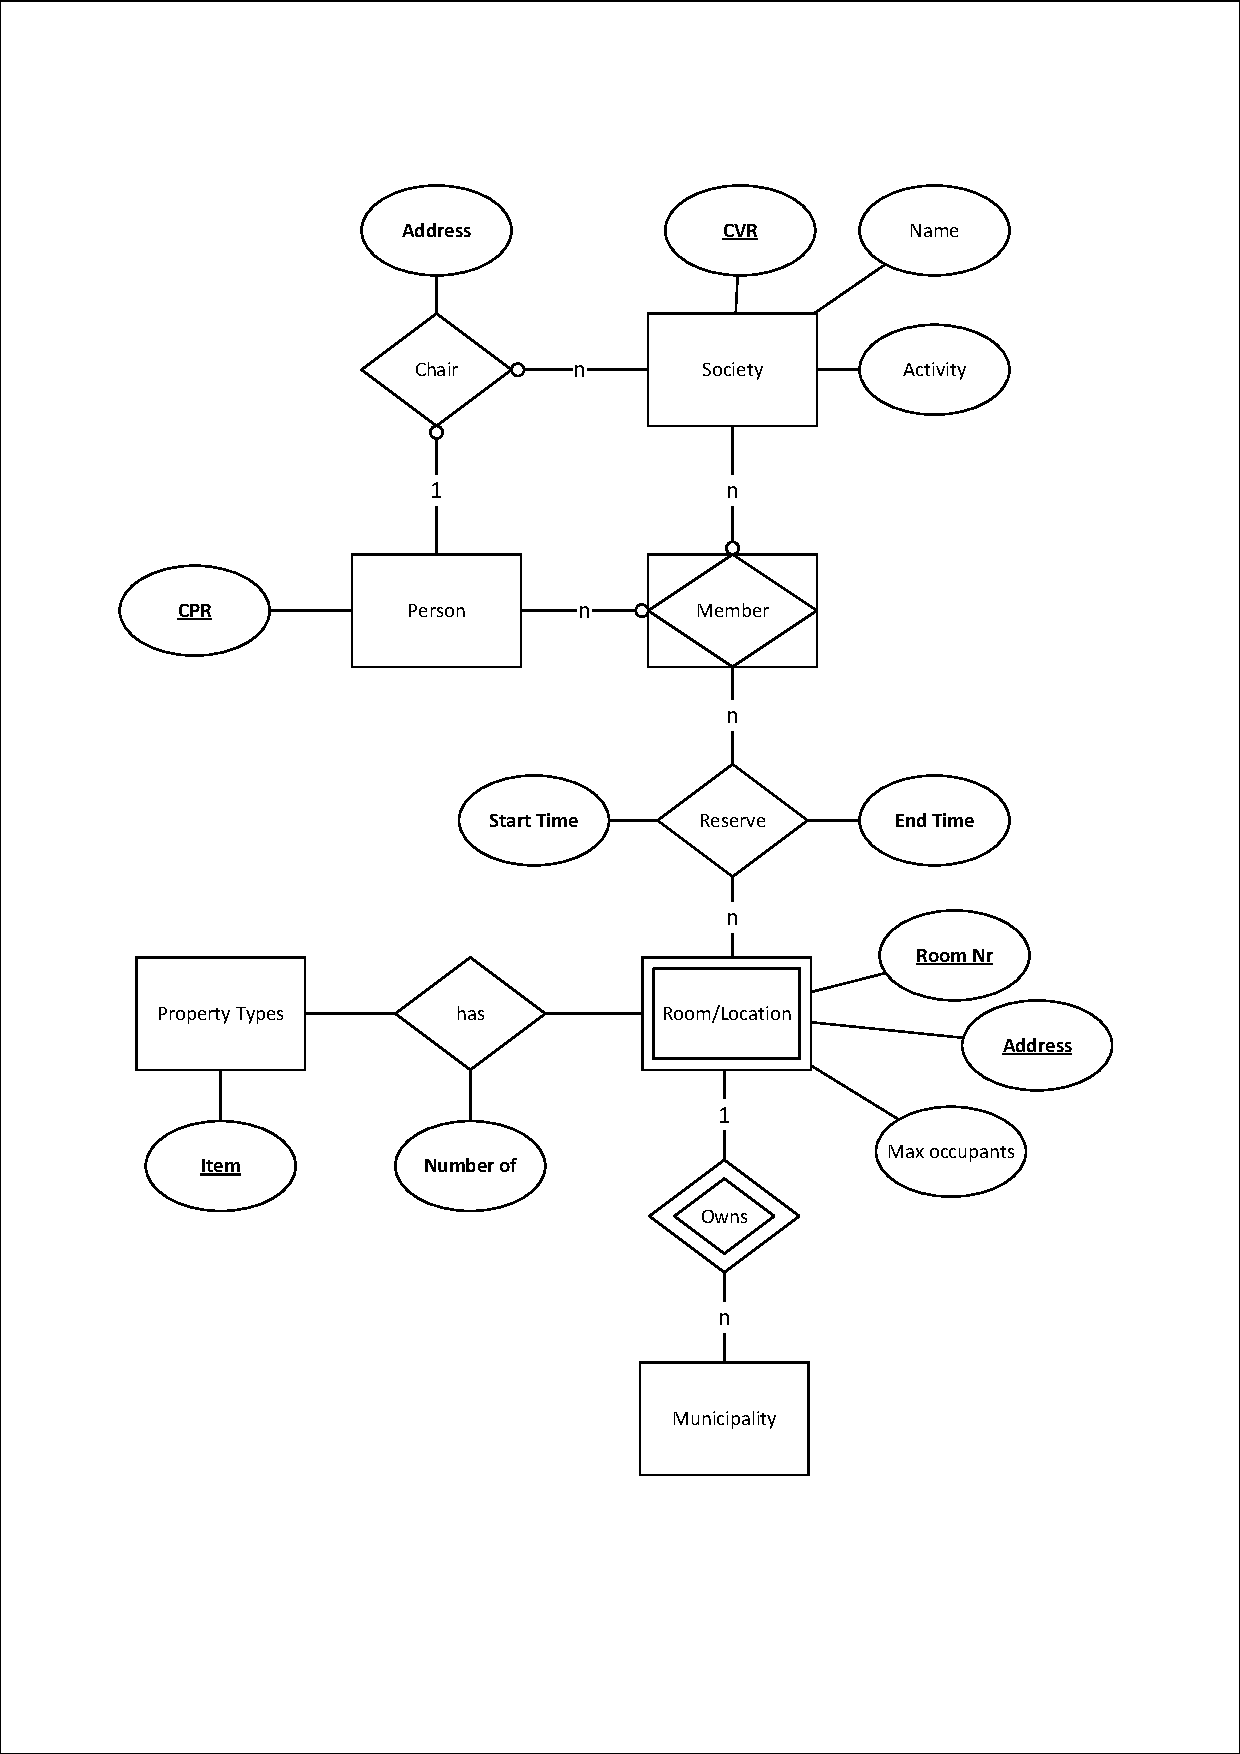
\includegraphics[scale=.66]{./ER diagram 1.pdf}
\end{figure}

\newpage
